% \begin{wrapfigure}[19]{r}{0.26\textwidth}
\begin{figure}[H]
%   \vspace{-0.6cm}
  \begin{center}
    \begin{subfigure}[b]{0.26\textwidth}
        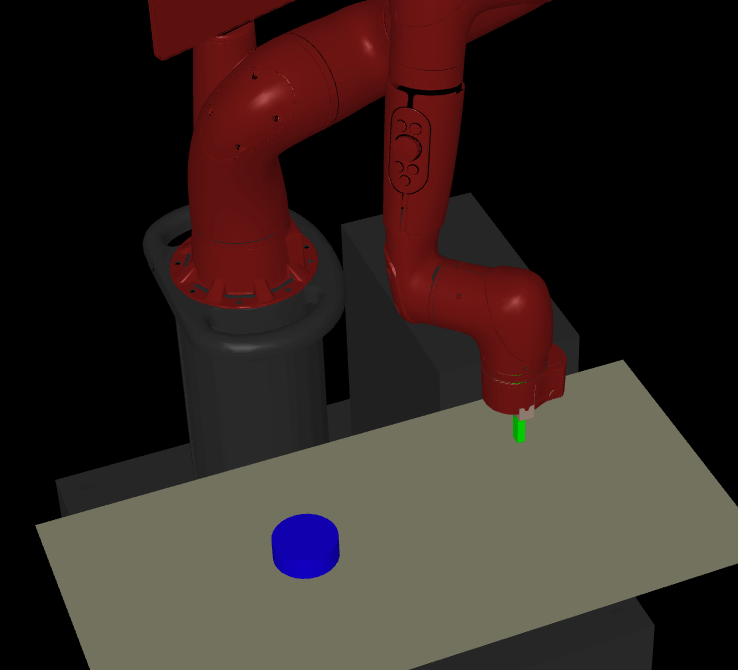
\includegraphics[width=0.99\textwidth,trim={5cm 0 5cm 0},clip]{awac/figures/imgs/sawyer_push.png}
    \end{subfigure}
    \hspace{0.03\textwidth}
    \begin{subfigure}[b]{0.45\textwidth}
        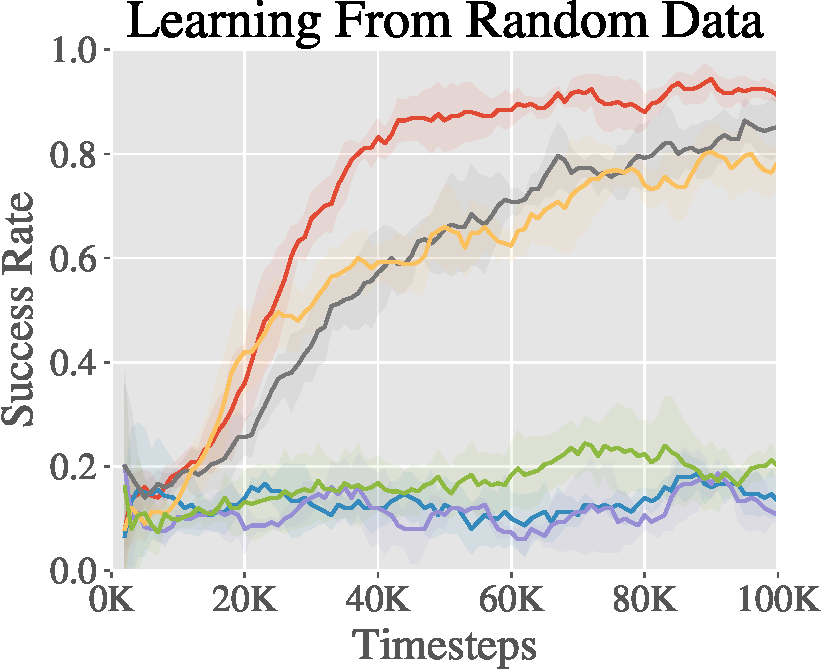
\includegraphics[width=0.9\textwidth]{awac/figures/rig/pusher_random-crop.pdf}
        
        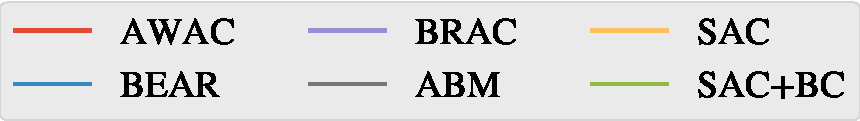
\includegraphics[width=0.9\textwidth]{awac/figures/rig/pusher_random_legend-crop.pdf}
    \end{subfigure}
  \end{center}
  \vspace{0.1cm}
  \caption{
%   \footnotesize{
  Comparison of fine-tuning from an initial dataset of suboptimal data on a Sawyer robot pushing task.
%   }
  }
  %\vspace{-0.5cm}
 \label{fig:gcrl}
\end{figure}
% \end{wrapfigure}